\chapter{Word Alignment}\label{chap:word-alignment}

We now reach the core of my thesis, computing word alignments using the novel method \enquote{SimAlign} \autocite{jalili-sabet-etal-2020-simalign} and evaluating it against two baseline methods, I shall give a short introduction to the topic of word alignment and explain the mechanisms behind statistical word alignment and  similarity/word embedding-based word alignment.

\section{Introduction}
Following the success of statistical models in sentence alignment, word alignment was seen as a natural extension of that work. 
This work had two main goals: offer a valuable resource in bilingual lexicography and develop a system for automatic translation \autocite{brown-etal-1993-mathematics}. 

Word alignments are objects indicating for each word in a string in the target language \(f\) which word in the source language \(e\) it arose from \autocite{brown-etal-1993-mathematics}. 
In other words, it is a mapping of words in a string of the source language \(e\) to the words in a string of the target language \(f\) \autocite[84]{koehn2009}.

A simple example for an alignment for a pair of sentences from the corpus I compiled are the German sentence \emph{Die Beratungen sind kostenlos} \enquote{The consultations are gratuitous} and its Romansh counterpart \emph{Las cussegliaziuns èn gratuitas}. 


\begin{figure}[h]
\centering

\tikzmarknode{s0}{1\\ Die} \tikzmarknode{s1}{2\\ Beratungen} \tikzmarknode{s2}{3\\ sind} \tikzmarknode{s3}{4\\ kostenlos} 

\vspace*{1cm}

\tikzmarknode{t0}{Las\\1} \tikzmarknode{t1}{cussegliaziuns\\2} \tikzmarknode{t2}{èn\\3} \tikzmarknode{t3}{gratuitas\\4}
\begin{tikzpicture}[remember picture, overlay, scale=0.6, every node/.style={scale=0.6}]
\draw
(s0) -- (t0)
(s1) -- (t1)
(s2) -- (t2)
(s3) -- (t3)
;
\end{tikzpicture}
\caption[Word alignment example]{Example of a word alignment between two sentences in German and Romansh}
\end{figure}


In this example, each word in German is aligned to exactly one word in Romansh and the words follow exactly the same order, such that the resulting alignment is the set of mappings $\{1\to1, 2\to2,3\to3,4\to4\}$. 
Such alignments, in which each word in the source sentence is aligned to exactly one word in the target sentence, and in which the words follow the same order, are considered simple \autocite[85]{koehn2009}.

Things become more complicated when word order differs between languages or when several words in one sentence are mapped to one or several words in the other sentence. 
The latter gives rise to a variety of alignment types. 
A word in the target language may be aligned to several words in the source language (1-to-many alignment), or several words in the target language may be aligned to one word in the source language (many-to-1 alignment). 
Sometimes words in the target have no relation to the source (for instance in case of untranslatable words, or words that were omitted in the translation). 
In that case, they will be aligned to a special \texttt{NULL} token \autocite[85]{koehn2009}. 

%There is an assymetry in classical alignment models between the source and the target language. 
%Each target word is connected to exactly one source word; but source words can be linked to multiple target words or to no words at all. 
%This difficulty will not bother us 

In order to deal with these challenges of different word order and alignments that are not 1-to-1 alignments, \textcite{brown-etal-1993-mathematics} developed their pipeline of translation models, the IBM Models 1-5.

\section{Overview of Methods}
I shall now give a quick explanation of word alignment methods, namely of the IBM Models, and of SimAlign, a similarity-based alignment model that uses  word embeddings. 
Since I am not a mathematician, I will not go into the mathematics of these models. 
I will rather attempt to explain their \emph{modus operandi} in a more intuitive way, so as to to allow the reader some basic understanding of the mechanics behind the scenes.

\subsection{IBM Model 1}
\label{sec:ibm-model-1}
The IBM models are translation models. 
They were developed in order to compute the conditional probability of a sentence in the target language $f$ given a sentence in the source langauge $e$: $P(f|e)$ \autocite{brown-etal-1993-mathematics}. 
In layman's terms, they compute how likely a given sentence in the target language is a translation of a sentence in the source language.
By modeling these probabilities, the models can generate a number of different translations for a sentence. 
However, there are infinitely many sentences in a language and most sentences occur, even in large corpora, only once. 
This makes the task of modeling the probability distribution for full sentences hard and not promising. 
Instead, the problem is broken up into smaller steps: the model models the probability distributions for individual words---it computes how likely a word in one sentence is a translation of a word in that sentence's translation. 
The IBM Model 1 is therefore based solely on modeling the probability distributions of lexical translations, i.e., of individual words \autocite[88]{koehn2009}.

\subsubsection{Incomplete Data}
There is, however, a problem. 
We can compute the probability distributions of lexical translations given their counts. 
That is, by counting how often a word $s^e_i$ in the sentence $s_e$ in language $e$ was translated as a word $s^f_j$ in a sentence $s_f$ in language $f$, we can compute the desired probability distributions. 
Take for example a set of German-English sentence pairs. By counting how many times the German word \emph{das} was translated as \emph{the}, how many times it was translated as \emph{that}, etc., we can compute each word's translation probability distribution. 
With these individual probability distributions we can compute the likelihood of a sentence in language $f$ being a translation of a sentence in language $e$ \autocite[88]{koehn2009}.
Unfortunately, while sentence alignment is a relatively easy task (at least for well-structured texts), and while sentence aligned parallel corpora are not hard to compile or come by, we do not know which words correspond to which words in the sentence pairs. In other words, we do not know \emph{a priori} how each word in the source sentence was translated, which means we cannot compute the counts for the probability distributions.

This problem, dubbed as a \emph{chicken and egg problem}, is basically the following: If we had word alignments, it wouldn't be a problem to estimate the lexical translation model and compute the probability distributions for words and sentences; 
And if we had a model, we could easily estimate the most likely correspondences between words in the source and the target sentences. 
Unfortunately, we have none of the above \autocite[88]{koehn2009}.


\subsubsection{EM Algorithm} 
In order to solve the problem of incomplete data, an iterative learning algorithm, the \acrfull{em} algorithm comes into play. 
The EM algorithm is mathematically intricate. 
I shall try to explain in simple words the idea behind it. 

In the very first iteration, the values of the model parameters are unknown and are initialized with a uniform distribution. 
This means all words are equally likely  translations of each other.
Then, in the estimation step, the model is applied to the data to compute the most likely alignments. 
In the maximization step, the model is learned from the data based on counts collected from it. 
The algorithm counts co-occurrences of words in the source and the target languages, which are then weighted with the probabilities that were computed in the estimation step.
These weighted counts are used to compute again the probabilities in the next estimation step. 
These two steps, estimation and maximization, are then repeated until convergence---until a global minimum has been reached \autocites[88-92]{koehn2009}{brown-etal-1993-mathematics}.

In simple words, the model does not know in the beginning which words in the source language correspond to which words in the target language. 
In the very first iteration, all alignments are equally likely---any word in a sentence in the target language is equally likely a translation of any word in the source language.
In order to find the most probable correspondences (or alignments), the model counts how often words are aligned with each other, that is, how often they co-occur in parallel sentences (maximization step). 
These counts are weighted with the probabilities computed in the previous estimation step to refine the values in the next estimation step. 
Likely links between words are strengthened, while less likely links are weakened. 
This goes on until the model converges and the most likely word alignments have been learned by the model. 

\subsection{Higher IBM Models}
Without going too much into detail, I will shortly mention the other IBM models, Models 2-5. 

Model 1 makes the unrealistic assumption that all connections for each position are equally likely. 
This means that word order is not modeled by Model 1. 
Simply put, the word order does not influence the likelihood of word alignments.
Therefore, Model 2 \emph{does} depend on word order. 
It adds an explicit model for alignment based on the absolute positions of the source and the target words \autocites{brown-etal-1993-mathematics}[99]{koehn2009}.

Model 3 adds a probability distribution of the number of words a source word is usually translated to (dubbed \emph{fertility}). 
It is able to model alignments of types other than 1-to-1 \autocite[100]{koehn2009}. 
% In Model 4, the probability of alignments depends in addition on the positions of any other target words that are connected with the same source word.

Models 4 and 5 add more complexity and take into account for instance the positions of any other target words that are connected with the same source word \autocite{brown-etal-1993-mathematics}, since words that are next to each other in the source sentence tend to be next to each other in the target sentence (large phrases tend to move together as units) \autocite[107]{koehn2009}.

Models 1-4 serve as stepping stones towards the training of Model 5. 
Model 1 has a simple mathematical form and a one unique local minimum, which means the parameters learned by it do not depend on the starting point\footnote{The other models have several minima; this means according to the starting parameters, different minima can be arrived at.}. 
The estimates learned by Model 1 are used to initialize the training of Model 2, those of Model 2 are used to initialize Model 3, and so on, and so forth---each model is initialized from the parameters of the model before it. 
This way, the estimates arrived at by the end of training of Model 5 do not depend  on the initial estimates of the parameters for Model 1 \autocite{brown-etal-1993-mathematics}. 

These models have been playing a key role in word alignment tasks and in statistical machine translation. 
Put together in a pipeline of models, they serve as the groundwork for Giza++, a toolkit for training word-based translation models. 
Using these alignments, phrase alignments can be learned in order to train a statistical phrase-based machine translation \autocites{och-ney-2000-improved,och-ney-2003-smt}

% In other words, while the higher models may converge at different minima, Model 1 will always converge at the same minimum, regardless of the parameters it was initialized with. 
% Passing the parameters learned by each model to the next model allows us to not simply start training with some random parameters, 



\section{Word Embeddings}
\label{sec:word-embeddings}
A different approach to word alignment is based on similarity between words, which is in turn computed using word embeddings. 
But what are word embeddings?
 

\subsection{Excursion: Words}
Before we discuss word embeddings, I would like to write a few words about words and their meanings.

Words are actually an arbitrary way to split linguistic material into units. 
What we refer to as words are usually units separated by a whitespace in writing, but the use of whitespaces is arbitrary and inconsistent. 
There is no real phonetic motivation for splitting units into words. 
Some single words sound exactly like two other words (\emph{a maze} sounds like \emph{amaze} and \emph{in sight} like \emph{incite}). 
The words \emph{someone} and \emph{anyone} are written as one word, while \emph{no one} is written as two words, although there is obviously no difference in character between them \autocite[92-95]{Jespersen1924}.

For the sake of simplicity, I will stick to the term \emph{word}, referring to any linguistic unit, made up of one or several morphemes (or words), divided in written form by whitespaces from its neighboring units.

\subsubsection{Meaning of Words}
The question of describing the meanings of words is an entire field: semantics. But already in his posthumously published work \emph{Cours de linguistique générale} (\enquote{Course in General Linguistics}) from 1916, the Swiss linguist and semiotician, Fredinand de Sassure, came to an important conclusion. 
Linguistic elements receive their value only by being arranged in a sequence, which de Saussure calls \emph{syntagm}: 
\enquote{A term in the syntagm acquires its value only because it stands in opposition to everything that precedes or follows it, or to both.} \autocite[123]{de-saussure-1959-course} 

Additionally, each term in the syntagm, in the sequence of terms, has associative (or \emph{paradigmatic}) relations. 
These relations reside in the memory of the speakers. 
For instance the German word \emph{zudrehen} \enquote{close something by turning} unconciously calls to mind related words, such as other words beginning with \emph{zu-}: \emph{zumachen} \enquote{close}, \emph{zumauern} \enquote{wall something up}, \emph{zuklappen} \enquote{close something shut}. 
But also words with the verb \emph{drehen}: \emph{aufdrehen} \enquote{turn open}, \emph{verdrehen} \enquote{twist, contort}, etc. etc. \autocite[122-127]{de-saussure-1959-course}\footnote{Examples are my own.}.

Each term in the syntagm stands in opposition not only to the preceding and following parts in the syntagm, but also to terms in the paradigm, which are called to mind by the associative series. 
The meaning, or rather value of words, is a result of an intersection of two axes---the syntagmatic, the horizontal axis, and the paradigmatic axis, the vertical axis.

Take, for instance, the sentence \emph{I am drinking coffee}. The word \emph{coffee} gets its  \textbf{syntagmatic} value from the perceding word \emph{drinking}, which stands in \textbf{paradigmatic} opposition to other words (\emph{plant}, \emph{grow}) which would give \emph{coffee} a different meaning.
We know that by \emph{coffee} a hot-drink is meant, because it follows the verb \emph{drink}. In the sentence \emph{I grow coffee} it would mean a plant or a tree, in \emph{I bought one pound of coffee} it would mean beans, and in \emph{coffee ice-cream} it would describe a flavor.

The Austrian-British philosopher, Ludwig Wittgenstein, summed up the meaning of the word \emph{meaning} (German \emph{Bedeutung}) in two sentences in his Philosophical Investigations, no. 43:


\begin{displayquote}\emph{
Man kann für eine große Klasse von Fällen der Benützung des Wortes »Bedeutung« – wenn auch nicht für alle Fälle seiner Benützung – dieses Wort so erklären: Die Bedeutung eines Wortes ist sein Gebrauch in der Sprache.}\footnote{{For a large class of cases of the use of the word \emph{meaning}---and maybe for all of its use cases---one could explain the word as follows: The meaning of a word is its use in the language.}} {\interfootnotelinepenalty10000 \footnote{\url{https://www.wittgensteinproject.org/w/index.php?title=Philosophische_Untersuchungen\#43}}}
\end{displayquote}

\subsection{Word Embeddings}
These ideas, which were further developed by linguists in the 1950's, namely that a word can be defined by its environment or distribution, i.e., by its set of contexts in which it occurs and its grammatical environments, is the inspiration for what is called vector semantics.  
The idea of vector semantics is to represent a word as a point in some $n$-dimensional vector space. 
These vectors are called \emph{embeddings}. 
There are different ways and versions of word embeddings, but in each case the values of the vectors are based in some way on counts of neighboring words \autocite[98-99]{jurafsky-2019}.

\subsubsection{Neural Language Models}
One version of word embeddings comes from neural language models.
Language modeling is the task of assigning probabilities to a sequence of words, that is, modeling how likely it is that a sequence of words in a language would be uttered/written by a speaker of that language \autocite[181]{koehn2009}. 
In practice, the task of a language model is predicting upcoming words from prior word context \autocite[137]{jurafsky-2019}.

In a neural language model, the modeling is done using a neural network. 
Without going too much into detail, a neural network is a complex non-linear function. 
It is made up of layers, which are vectors, and weights, which are matrices. 
The numbers (a vector) from each layer are passed on to the next layer by multiplying it with the weights (a matrix) between the layers using matrix multiplication. 
The vector resulting from this matrix multiplication (usually passed through some non-linear activation function), is the next layer in the neural network. 
The output of a neural network can be  a single value, as in the cases of a binary classification task, in which the output is either 0 or 1, but it can also be a vector representing some probability distribution.

In the course of the training of a neural language  model, i.e., while the neural network learns the probability distributions for words given its neighboring words, the parameters for the weights are learned. 
The weights connecting the input layer with the first hidden layer are our said word embeddings. 
When inputting a word into the network (in form of a one-hot vector), we can get its vector representation, i.e., its embedding, from the so-called embedding layer. 
Since this representation is conditioned on context, similar words should have similar embeddings \autocite[104-105]{koehn-2020}.

\subsubsection{Neural Embeddings}

There are different ways for learning word embeddings. 
Two of the most popular methods are \emph{word2vec} (actually made up of two different methods) and \emph{GloVE}. 
These methods are simpler than neural language models \autocite[111]{jurafsky-2019}; their main goal is to learn high quality word vector representations, not to generate language.

\subsubsection{Sub-words}\label{sec:subwords}
Due to computational limitations, neural language models usually have a fixed vocabulary size. 
This means that even if we had some hypothetical corpus which contains all the words in a language, the model will still not be able to \enquote{learn} all these words. 
Some words will remain out-of-vocabulary.
There are different ways for dealing with this limitation in vocabulary size, i.e., with rare words. 
One way is to split words into sub-word units. 
There are different algorithms for splitting words. 
mBERT uses an algorithm called WordPiece \autocites{wu-2016-wordpiece,delvin-chang-2018-bert} and XLM-R uses BPE \autocites{conneau-etal-2020-xlm,sennrich-etal-2016-neural}.


\subsection{Word Similarity}
\label{sec:word-similarity}
If words are represented by vectors, we need a measure for taking two such vectors and determining how similar they are. 
The most common similarity metric is the \textbf{cosine similarity}---measuring the angle between the vectors. 

Again, without going into too much mathematical details, using the dot product for measuring similarity, i.e., multiplying the vectors with each other, favors long vectors. Long vectors are vectors with high values in each dimension, which represents the frequency of words. 
This means more frequent words would have higher values, but we are interested in measuring the similarity between words regardless of their frequency.
To solve this problem, we need to \textbf{normalize the dot product} by dividing it by the lengths of the vectors. 
Thus, the cosine similarity metric between two vectors $\mathbf{v}$ and $\mathbf{w}$ can be computed as:

\begin{equation}
	\text{cosine}(\mathbf{v}, \mathbf{w}) =
	\frac{
	\mathbf{v} \cdot \mathbf{w}
	}{|\mathbf{v}||\mathbf{w}|}
	=
	\frac{
	\sum_{i=1}^N v_i w_i
	}
	{
	\sqrt{\sum_{i=1}^N v_i^2} \sqrt{\sum_{i=1}^N w_i^2}
	}	
\end{equation}

With $\sum_{i=1}^Nv_iw_i$ being the dot product of the vectors $\mathbf{v}$ and $\mathbf{w}$, and $\sqrt{\sum_{i=1}^N v_i^2}$ and $\sqrt{\sum_{i=1}^N w_i^2}$ being the lengths of the vectors $\mathbf{v}$ and $\mathbf{w}$, respectively \autocite[103-104]{jurafsky-2019}.

The cosine similarity returns a value between $-1$ and $1$. 
The highest  similarity is \(1\): the vectors are parallel and pointing in the same direction. 
If it is $0$, the angle between the vectors is a $90^\circ$ angle. 
The lowest similarity is $-1$: the vectors point in opposite directions.

\subsection{Multilingual Word Embeddings}
\label{subsec:multilingual-word-embeddings}
There are also methods for computing multilingual word embeddings. 
Multilingual word embeddings are word embeddings for words in different languages that share the same vector space. 
This can be achieved by learning word embeddings for each language separately on monolingual data, and then mapping these embeddings to a shared vector space \autocite{artetxe-etal-2018-robust}. 
When multilingual word embeddings are learned, the embeddings of the different languages have to be aligned to each other, such that they share similar geometrical shapes and are aligned across the same axes, in order for vectors of similar words across different languages to be next to each other in the vector space \autocite[220-223]{koehn-2020}. See Figure~\ref{fig:embedding-alignment}.


\begin{figure}[ht]
\centering
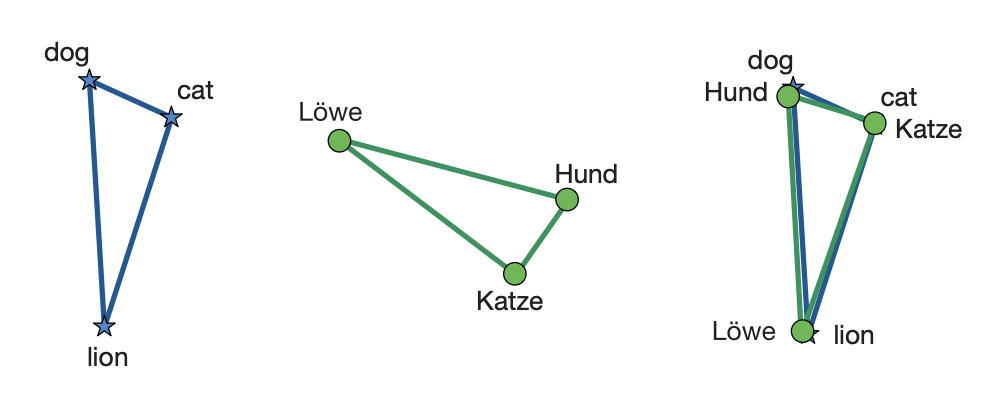
\includegraphics[width=0.9\textwidth]{graphics/embedding-alignment.png}
\caption[Matching up the geometric shape of embedding spaces of words in English and German]{Matching up the geometric shape of embedding spaces of words in English and German. 
Taken from \cite[223]{koehn-2020}}.
\label{fig:embedding-alignment}
\end{figure}

Multilingual word embeddings can also be extracted from a multilingual language model \autocite{jalili-sabet-etal-2020-simalign}.

The idea behind multilingual word embeddings is that two equivalent words in different languages should have a similar distribution, thus their vector representations should also be similar \autocite{artetxe-etal-2018-robust}. 

\subsection{Summary}
Word embeddings are vector representations of words learned by a neural language model or by a more simple embeddings model. 
These vectors' dimensions usually range between 100 and 1000 dimensions. 
Similar words (words that appear in the same context) have similar word embeddings. 
To measure word similarity, we measure the similarity between their embeddings using the cosine similarity.
Multilingual word embeddings are word embeddings for words in different languages  sharing the same vector space. 
Similar words in different languages should have similar embeddings.

\section{Similarity-Based Word Alignment}

% Without going too much into details, when a simple neural language models learns the probabilty distributions for words given all the previous words, the weights in the hidden layer are adapted. 
% We can then use the language model not for generating language, but extract the weights for a specific word from the inner layer, which are an $n$-dimensional vector.
% We call this vector word embedding.

% It has been shown that words that occur in similar contexts have similar word embeddings. 
% This vector similarity can be measured with the cosine similarity.

If similar words in different languages have similar embeddings, these embeddings can be  leveraged in order to find word alignments using a similarity matrix, without the need for parallel training data. This is the idea that forms the basis of SimAlign \autocite{jalili-sabet-etal-2020-simalign}.

\subsection{Method}
\label{subsec:simalign-method}
SimAlign takes two parallel sentences $s_e$ and $s_f$ of lengths $l_e$ and $l_f$ in languages $e$ and $f$. 
For this sentence pair a \emph{similarity matrix} is defined as $S \in [0,1]^{l_e\times l_f}$. 
It is a matrix the size of the lengths of the sentences. Each cell in the matrix will be filled with a value between 0 and 1, returned from a function measuring similarity between the embeddings of two words. 
This means that for each combination of two words from sentence $s_e$ and sentence $s_f$, their similarity measure is filled into the corresponding cell in the matrix (Figure~\ref{fig:sim-matrix}).
From this similarity matrix $S$, a binary alignment matrix $A \in \{0,1\}^{l_e \times l_f}$ is extracted. 
The cell $A_{ij}$ in the alignment matrix $A$ will be filled with 1 (which means $i$ and $j$ will be aligned) if the word $s_i^e$ in the sentence $s_e$ is the most similar to the word $s_j^f$ in the sentence $s_f$ and vice versa (Figure~\ref{fig:al-matrix}).



\begin{figure}
\[
	\begin{array}{rl|c|c|c|c}
& &1 & 2 & 3 & 4\\
& &\text{Ich} & \text{liebe} & \text{ja} & \text{Äpfel} \\
\hline
1 & \text{I} & 0.9 & 0.2 & 0 &0.2 \\ 
\hline
2 & \text{love} & 0.1 & 0.9 &0 & 0.1 \\
\hline
3 & \text{apples } & 0.1& 0.1 & 0 & 0.9\\
\end{array}
\]
\captionsetup{width=.6\linewidth}
\caption[Similarity matrix]{Similarity matrix $S \in [0,1]^{l_e \times l_x}$, filled with values between 0 and 1 corresponding to the similarity measure between the embeddings of the words. 
The values are fictive.}
\label{fig:sim-matrix}
\end{figure}

\begin{figure}
\[
	\begin{array}{rl|c|c|c|c}
& &1 & 2 & 3 & 4\\
& &\text{Ich} & \text{liebe} & \text{ja} & \text{Äpfel} \\
\hline
1 & \text{I} & 1 & 0 & 0 & 0 \\ 
\hline
2 & \text{love} & 0 & 1 &0 & 0 \\
\hline
3 & \text{apples } & 0& 0 & 0 & 1\\
\end{array}
\]
\captionsetup{width=.6\linewidth}
\caption[Alignment matrix]{Alignment matrix $A \in \{0,1\}^{l_e \times l_f}$ extracted from the similarity matrix S. The two most similar words in row $i$ and column $j$ of S will receive a score of 1; the rest 0.}
\label{fig:al-matrix}
\end{figure}
\begin{figure}
\centering

\tikzmarknode{s0}{Ich} \tikzmarknode{s1}{liebe} \tikzmarknode{s2}{ja} \tikzmarknode{s3}{Äpfel} 

\vspace*{1cm}

\tikzmarknode{t0}{I} \tikzmarknode{t1}{love} \tikzmarknode{t2}{apples} 
\begin{tikzpicture}[remember picture, overlay, scale=0.6, every node/.style={scale=0.6}]
\draw
(s0) -- (t0)
(s1) -- (t1)
(s3) -- (t2)
;
\end{tikzpicture}
\caption{The resulting word alignment}
\label{fig:resulting-alignment}
\end{figure}


That is, a cell $A_{ij}$ in the matrix $A$ is set to 1 if:
\[
	(i= \arg \max_l S_{l,j}) \land (j=\arg\max_l S_{i,l})
\]

% The expression $\arg \max_l S_{l,j}$ returns the row $i$ in the column $j$ of the matrix $S$ with the highest value. 
% If the current $A_i$ equals to the $\arg\max$ expression \textbf{and} 

If all entries in a row $i$ or a column $j$ of S are 0 (as is the case in column 3 of Figure~\ref{fig:sim-matrix}), $A_{ij}$ will be set to 0.
The resulting alignment can be seen in Figure~\ref{fig:resulting-alignment}.

This basic method is referred to in \textcite{jalili-sabet-etal-2020-simalign} as \textbf{Argmax}. Mutual argmaxes can be rare, which is why for many sentences Argmax only identifies few alignments. 
To remedy this, Argmax is applied iteratively in a method called \textbf{Itermax}. 
In each iteration, the model focuses on still unaligned pairs and tries to align them. 
Further, if the similarity with an already aligned word is very high, the model can add another alignment edge. 
This allows for one word to be aligned to multiple other words, i.e., create 1-to-many alignments.

Argmax finds a local optimum and Itermax is a greedy algorithm. 
There is a third alignment method, called \textbf{Match}, which finds global optima. 
The alignments generated with the Match method are inherently bidirectional (the source is aligned to the target and the target is aligned to the source)\footnote{\textcite{jalili-sabet-etal-2020-simalign} don't elaborate on the relevance  of the notion of source and target sentences.}.

For the task of word alignment, SimAlign can use multilingual embeddings which were learned in advance from monolingual data and then mapped to a shared vector space. 
SimAlign can also use, out-of-the-box, the embeddings from two multilingual language models: mBERT, which is a version of BERT \autocite{delvin-chang-2018-bert} trained on 104 languages\footnote{\url{https://github.com/google-research/bert/blob/master/multilingual.md}}, and XLM-RoBERTa base, trained on 100 languages \autocite{conneau-etal-2020-xlm}. 

However, none of these models has \enquote{seen} Romansh, i.e., Romansh is not part of the training data for these models. 
But multilingual models were shown to generalize even for unseen languages. 
mBERT, for instance, achieves reasonable results out-of-the-box (without further training) on unseen languages in a variety of tasks such as \acrfull{ner} and \acrfull{pos} tagging \autocite{pires-etal-2019-multilingual}. 
There is therefore good reason to expect that SimAlign would also work for aligning words in sentence pairs with Romansh.


\subsection{Summary}
By measuring the similarity between multilingual word embeddings, word alignments for sentence pairs in the languages the models were pre-trained on can be computed. 
Multilingual embeddings can be learned from monolingual data, and thus word alignment can be computed even in low-resource scenarios, i.e., in scenarios where parallel data is scarce, which makes similarity-based word alignment a competitive method against statistical methods. 

Traditional statistical methods such as the IBM Models \autocite{brown-etal-1993-mathematics} and their implementations, such as GIZA++ \autocite{och-ney-2003-smt} or fast\_align \autocite{dyer-etal-2013-simple} require a large amount of parallel data to perform well.
The quality of the alignments deteriorates quickly when the size of data diminishes\footnotemark. 

\footnotetext{In \textcite{och-ney-2000-improved}, the \acrfull{aer} for aligning words in 1.5M sentence pairs is $9.4\%$. 
When aligning words in only \numprint{50000} sentences, the \acrshort{aer} goes up to $15.6\%$ (see Table 4 in \textcite{och-ney-2000-improved}).}

In experiments done by \textcite{jalili-sabet-etal-2020-simalign}, their similarity-based word alignment method, when using embeddings extracted from mBERT or XLM-R, outperforms any state-of-the-art statistical method for the languages Czech, German, French and Hindi, paired with English. 
However, all of these languages were included in mBERT's and XLM-R's training data. 
\textcite{jalili-sabet-etal-2020-simalign} emphasize the advantage of their method being high performance also in the case of little  parallel data.

In the following two chapters I will describe the creation of a gold standard (Chapter~\ref{chap:gold-standard}) in order to answer my research question and test \textbf{whether SimAlign performs just as well on data unseen by said language models, specifically for the language pair German-Romansh} (Chapter~\ref{chap:results}).



